\documentclass[oneside,a4paper,english,links]{article}
%
\usepackage{graphicx}
\usepackage{amsmath,amsfonts}
\usepackage{url}
\usepackage{subfig}
\usepackage{ amssymb }

\newcommand{\rodrigo}[1]{\authnote{Rodrigo}{#1}}

\title{GPU implementation of the sandbox multifractal method}

\author{Rodrigo Baravalle}

\begin{document}

\maketitle
\begin{center}
\small{Laboratorio de Sistemas Din\'amicos y Procesamiento de Informaci\'on, FCEIA, Universidad Nacional de Rosario - CIFASIS - CONICET}\\
\small{Riobamba 250 bis, 2000, Rosario, Argentina}\\

\texttt{baravalle@cifasis-conicet.gov.ar}\\
\texttt{\url{http://www.cifasis-conicet.gov.ar/index.php?grupo=4}}
\end{center}

\begin{abstract}
Adequate image descriptors are fundamental in image classification and object recognition. Main requirements for image features are robustness and low dimensionality which would lead to low classification errors in a variety of situations and with a reasonable computational cost. 

Recently, the theory of fractal sets has shown to provide local image features that are both robust and low-dimensional. In this work we apply a multifractal feature extraction technique for bread crumb classification based on colour scans of slices of different bread types. Preliminary results show that fractal based classification is able to distinguish different bread crumbs with high accuracy. A GPU-based implementation would help to accelerate the spectrum calculation in order to make possible to implement it in real time.
\end{abstract}

\section{Introduction}
Fractal and multifractal analysis of images have proved to capture useful properties of the underlying material being represented. Characterisation of images using these features have been successfully applied in different areas, such as medicine \cite{Andjelkovic2008,Yu2011} and texture classification \cite{Wendt2009}. Through several procedures, it is possible to obtain different Fractal Dimensions (FD), each of them capturing a different property of the material ({\em e.g.}, void image fraction, rugosity).

For each material, the results obtained in the classification process are useful in quality measurements of real samples and also in the validation of synthetic representations of them. 

In this work we propose to employ the generalized multifractal dimensions, obtained through the sandbox multifractal spectrum, as descriptors for the classification of different bread types and for the discrimination between bread and non-bread images. The results of this feature extraction procedure show that the classifier presents good discrimination properties to distinguish between different bread images. In section 2 we briefly introduce the theory underlying fractal sets. In section 3 we describe the materials and methods employed in the classification. In section 4 we show the results obtained in the classification and we perform a robustness analysis of the method. In section 5 we show the GPU based implementation. In section 6 we summarise the conclusions.

\section{Multifractal analysis}
Some elements in nature show fractal features or auto similarity. The fractal dimension is an exponent which relates the statistical auto similarity of the object at different scales. On the one hand, deterministic fractals are characterized by the same FD at all scales. They are called {\em monofractals} (for instance, Koch Curve, Sierpinsky triangle). On the other hand, {\em multifractals} \cite{Mandelbrot89} are characterized by a set of FDs depending on the scale. It is assumed that these structures are composed by different fractals coexisting simultaneously.

\subsection{Sandbox Method}
This method was introduced in \cite{Tel89} and it is useful to obtain generalized multifractal dimensions. If working with images, we first need to binarise the image, and then, $N$ points belonging to the structure ({\em i.e.}, regions with white pixels) should be randomly selected, counting for each point the number of white pixels inside a box of diameter $R$, centred at the point. The generalized sandbox dimension of order $q$ is obtained as \cite{Bert94}

\begin{equation}
D_{q} = \lim_{R\rightarrow0}{\frac{1}{q-1} \frac{\log \bigg \lbrack\frac{1}{N}\displaystyle \sum_{i=1}^{N}{p_{i}^{q-1}}\bigg \rbrack}{\log R}},
\label{eqn:eqn1}
\end{equation}

where $p_{i}$ is the number of points in the box of radius $R$ centred at the point $i$. An average is made over the $N$ points. Equation (\ref{eqn:eqn1}) can also be stated as

\begin{equation}
D_{q} = \lim_{R\rightarrow0}{D_{q}(R)}.
\end{equation}

In practice we perform a linear fit between the values of $D_{q}(R)$ and $R$ for $R$ in $[R_{min}, R_{max}]$. In this work, we apply this method to obtain a feature vector, setting different values of $q$ for each image, so then we can use it in classification tasks.

\section{Materials and Methodology}

\subsection{Image acquisition}
Twenty images of four different bread types ({\em lactal}, {\em baguette}, {\em salvado} and {\em sandwich}), counting $80$ images, were obtained using an electric slicer. Images showed a resolution of $380 \times 380$ pixels (the maximum possible area for the four bread types). Then the images were converted to grey scale ($8$ bits) and binarised. In addition, $20$ images of each bread type were acquired with a digital camera, using the same spatial resolution, counting $80$ images. The illumination conditions of these images were different from that of the scanner in order to test for the robustness of the method. In Fig.~\ref{fig:camera} four examples of bread images from the camera are shown. 

\begin{figure*}[htb]
\centering
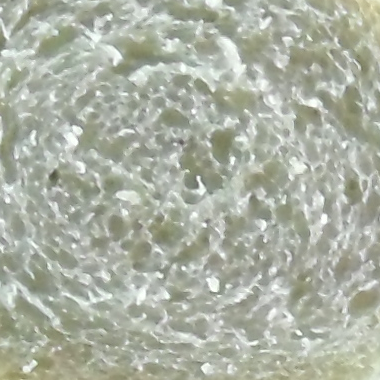
\includegraphics[scale=0.20]{imagenes/b}
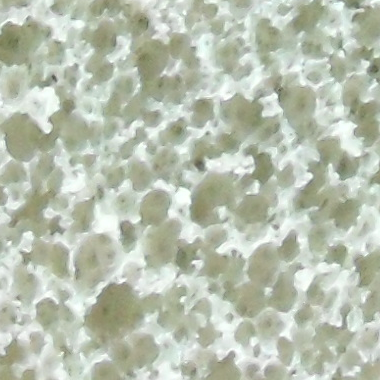
\includegraphics[scale=0.20]{imagenes/l19}
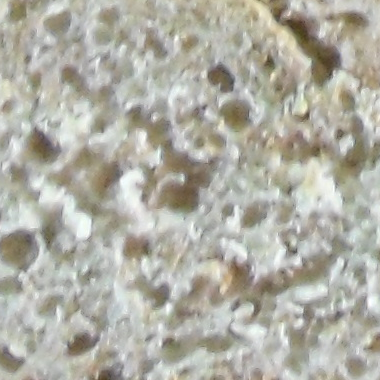
\includegraphics[scale=0.20]{imagenes/s7}
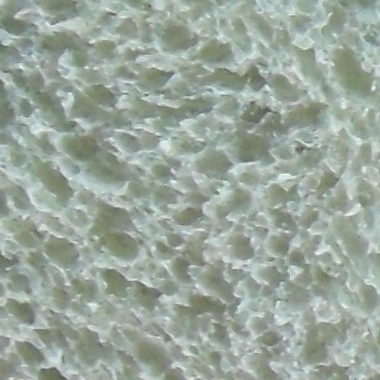
\includegraphics[scale=0.20]{imagenes/Sa14}
\caption{Digitalised images from a digital camera}
\label{fig:camera}
\end{figure*}

\subsection{Implementation}

The code of the algorithms for the computation of the sandbox method was written and run in python, with the help of the pyopencl library. The CPU actual implementation of the method takes approximately eight seconds per image to run, and depends in the number of selected points, the maximum window size and the number of fractal dimensions, but not on the image size.

\subsection{GPU-Implementation}
In the Sandbox implementation, the binarisationo algorithm applies a local thresholding for each pixel. The determination of the threshold can be done in parallel, since it does not depend on the rest of the pixels of the image. The CPU code is shown here:

\begin{verbatim}
for i in arrNx:
   for j in arrNy:
      if(mww(max(0,i-vent),max(0,j-vent),min(Nx-1,i+vent),min(Ny-1,j+vent),intImg)
          >= img.getpixel((i,j))*bias ): 
          im[j,i] = 255
\end{verbatim}

For each pixel image, if the mean of the pixels intensities in a window centered at the pixel is greater or equal than the actual pixel multiplied by a parameter (bias), then the pixel appears as white in the binarised image. The next snippet of code shows the GPU version of it.

\begin{verbatim}
import pyopencl as cl
...
prg = cl.Program(ctx, """
   ...
   __kernel void white(__global int *intImg, __global int *img, __global int *dest,
          const int Nx, const int Ny, const int vent, const float bias) {
      int gidx = get_global_id(0);
      int gidy = get_global_id(1);
      int i = gidy;
      int j = gidx;
      if(mww(max(0,i-vent),max(0,j-vent),min(Nx-1,i+vent),min(Ny-1,j+vent),intImg,Ny) 
                 >= (float)img[j + i*Ny]*bias )
         dest[j+i*Ny] = img[j+i*Ny];
   }
""").build()

prg.white(queue, a.shape, intImg_buf, img_buf, dest_buf,
      np.int32(Nx), np.int32(Ny), np.int32(vent), np.float32(bias))
cl.enqueue_read_buffer(queue, dest_buf, im).wait()
\end{verbatim}

The pyopencl library lets the code be written as normal OpenCL code. Then it is passed to the library. The function enqueue\_read\_buffer allows to obtain the result into a python array.

Also, when calculating each dimension, we said that a mean needed to be calculated. The python code is:

\begin{verbatim}
for h in range(1,P+1):        
    d[h-1]= np.sum(map(lambda i: (i**q)/aux1,c[h-1]))
\end{verbatim}

Each row of the $c$ array is summed in the $d$ array (applying some extra computation to each element). A parallel sum reduction could be performed on it. Pyopencl provides routines to do it automatically on an array. Since we needed to make some computation on each element of the array before performing the sum, a map expression (which would be applied to each element) could be passed as an argument. Then, the reduce\_expr results $a+b$, indicating that a sum is expected in the resulting array. The parallel reduction code results:


\begin{verbatim}
# parallel reduction of the sum in c[h]
krnl = pyopencl.reduction.ReductionKernel(ctx, np.float32, neutral="0",
        reduce_expr="a+b", map_expr="pow(x[i],q)/aux1",
        arguments="__global float *x, float q, const int aux1")
\end{verbatim}

Then the kernel is applied to each row of the c array as follows:

\begin{verbatim}
for h in range(P):        
    a = np.array(c[h]).astype(np.float32)
    in_buf = cl.Buffer(ctx, mf.READ_ONLY | mf.COPY_HOST_PTR, hostbuf=a)
    dest_buf = cl.Buffer(ctx, mf.WRITE_ONLY, a.nbytes)
    # where to store results      
    a = pyopencl.array.to_device(queue,a)
    d[h] = krnl(a, np.float32(q), np.int32(aux1)).get()  
\end{verbatim}
\section{Results}
The analysis was performed varying the parameters of the method in order to better understand the speed-up introduced by the GPU implementation. Table \ref{table:tableFirstTest} shows times for CPU and GPU implementations.

\begin{table}[htb]
\centering
\begin{tabular}{|c|c|c|c|c|c|}
    \hline
    \# Fractal Dimensions & $10$ & $10$ & $10$ & $5$ \\
    \hline
    \# Points & $100$ & $1000$ & $2000$ & $2000$ \\
    \hline
    Time (CPU)  & $2.94s$ & $7.14s$ & $12.97s$ & $7.95s$\\
    \hline
    Time (GPU) & $1.76s$ & $2.48s$ & $4.31s$ & $3.4s$ \\
    \hline
\end{tabular}
\caption{Time for different parameters}
\label{table:tableFirstTest}
\end{table}


\section{Conclusions}

The GPU implementation shows that The use of the GPU can speed up the computation of the method. The GPU implementation of the algorithm performs between $2$ and $3$ times faster than the CPU code. Further improvement of the method can be achieved looking for bottlenecks in the CPU implementation.


\bibliography{bibliografia/bib}
\bibliographystyle{unsrt}
\end{document}
